\documentclass[UTF8]{ctexart}
\title{第六章 设计结果验证}
\author{陈登}
\date{\today}

\bibliographystyle{plain}
\usepackage{graphicx}
\usepackage{float}
\usepackage{amsmath}
\usepackage{geometry}
\usepackage{fontspec}
\usepackage{algorithm}
\usepackage{algorithmicx}
\usepackage{algpseudocode}
\usepackage{diagbox}

\geometry{a4paper,centering,scale=0.9}
\usepackage[format=hang,font=small,textfont=it]{caption}
\usepackage[toc,page,title,titletoc,header]{appendix}
\usepackage[nottoc]{tocbibind}

\begin{document}

\section{设计结果验证}

本章节主要根据各个层级的相关设计要求给出具体的各个模块设计仿真、综合结果。
主要包含几个部分的模块,8B/10B解码器模块,码群同步模块,初始化帧同步和初始化lane同步模块,数据流控制模块。

\subsection{8B/10B解码器}

\subsubsection{仿真}

设计完整功能的8B/10B解码器仿真结果如图\ref{fig:8b_10b_decoder_wave}所示。

\begin{figure}[H]
	\centering
	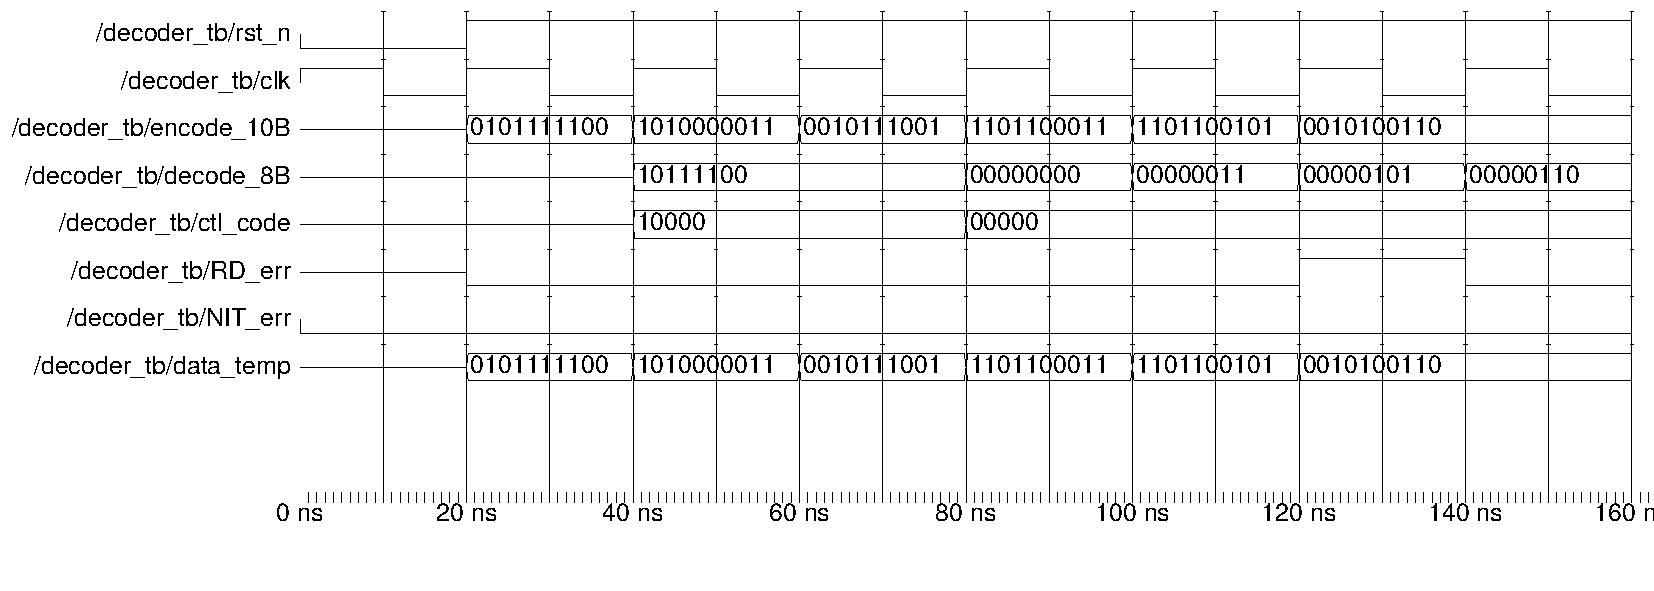
\includegraphics[width=18cm]{./img/8b_10b_decoder_wave.pdf}
	\caption{8B/10B解码器仿真结果}
	\label{fig:8b_10b_decoder_wave}
\end{figure}

可以看到,在复位信号启动后,输入端口收到了一系列的10B数据,并对这10B数据进行解码。
第一个接收到的数据为/K28.5/的10B编码,并且是极性呈正极性。
由于协议规定,8B/10B解码器初始的极性状态规定为负极性,所以最初传入的10B正极性数据并不会引起极性错误。
输入和输出之间由于有处理时延,所以通过时钟划定了一个octet时钟周期的时延。
第一个解码来的字符是/K28.5/,在ctl\_code端口可以看到编码为10000,其中置高的一位即表示/K/控制字符。
由于是控制字符,输出的具体解码数据并不重要。
第二个收到的字符也为/K28.5/的10B编码,不过由于之前一个10B编码表现为正极性,而此次收到的10B编码为负极性,并不会引起极性错误。
第二个字符的解码输出同第一个字符的解码输出,此时接收端极性为负极性。
第三个字符不再是控制字符,而是数据字符/D0.0/并且是一个中性极性的编码,并不改变当前极性,解码输出为00000000,解码正确。
第四个字符是数据字符/D3.0/,这是一个正极性的编码,与本地极性相反所以不会发生极性错误,本地极性翻转为正极性,解码输出为00000011,解码正确。
第五个字符是数据字符/D5.0/,这也是一个正极性的编码,与本地极性相同,所以接收端在此时RD\_err信号置高,表示发生极性错误,本地极性以刚接收到的数据极性为准,保持正极性,解码输出为00000101,解码正确。
由此可见,解码的正确与否与极性是否正确没有直接关系,极性错误并不会直接导致解码错误。
第六个字符是数据字符/D6.0/,这是一个负极性的编码,与本地极性相反,所以没有发生极性错误,解码输出为00000110,解码正确。

在这6个字符的测试序列中基本展示了8B/10B解码器的基本功能,包括了解码、极性错误判断和控制字符判断。
基本功能测试基本已经实现。

\subsubsection{综合}

综合过程一般分为四步:设定工艺库、读入RTL设计、进行综合、输出报告。
Linux下的DC可以通过GUI界面和命令行进行综合。
读入设计后可以通过GUI观察详细的门电路级电路,使用的器件既为器件库中所包含的器件。

综合完成后就可以得到详细的综合报告。
比较有价值的即面积报告、时序报告和功耗报告。
其中面积报告可以将每个子模块占用的面积总结出来,单位为平方微米($\mu m^2$);
时序报告会找到耗时最长的路径以表示电路最高的工作速度,单位为纳秒($ns$);
功耗报告即整体的功率损耗,单位为纳瓦($nW$)。

表\ref{tab:decoder_syn}详细比较了几种设计,其中括号里面的比例均为和新设计比较的比例,即视新设计具体之为100\%。

\begin{table}[H]
\centering
\caption{综合具体结果比较}
\label{tab:decoder_syn}
\begin{tabular}{|c|r|r|r|}

\hline

\diagbox{项目}{设计} & Classic & Actel & New \\

\hline

RD Cal Area($\mu m^2$) & & 665(99\%) & 675 \\

4B/3B Area($\mu m^2$) & & 369(148\%) & 249 \\

6B/5B Area($\mu m^2$) &				&	1184(172\%)	&	688		\\

\hline

Sum Area($\mu m^2$)				&	1570(97\%)	&	2218(138\%)	&	1612	\\

\hline

Total Cell Area($\mu m^2$)		&	1716(98\%)	&	2657(151\%)	&	1759	\\

\hline

Total Area($\mu m$)				&	16836(107\%)&	24497(156\%)&	15666	\\

\hline

Timing($ns$)					&	8.16 		&	9.97		&	9.54 	\\

Time Used($ns$)					&	5.84		&	4.03		&	4.46	\\

\hline

Frequency($MHz$)				&	171.2(76\%)	&	248.1(111\%)&	224.2 	\\

\hline

Cell Internal Power($nW$)		&	22.6(83\%)	&	31.0(114\%)	&	27.2 	\\

Net Switing Power($nW$)			&	42.8(80\%)	&	50.1(94\%)	&	53.3 	\\

\hline

Total Dynamic Power($nW$)		&	65.4(81\%)	&	81.1(101\%)	&	80.5 	\\

\hline

\end{tabular}
\end{table}

相较于Actel方法,新设计在频率上有11\%的减少,但是在面积上,无论是单元面积还是总面积都减少了近50\%的提升。
两者在功耗上几乎相同。
相较于传统方法,新设计在频率上有近25\%的提升,在单元面积上几乎相同,在总面积上减少了7\%。
但是在功耗上有近20\%的差距。

\subsection{码群同步}

\subsubsection{仿真}

设计完整功能的码群同步仿真结果如图\ref{fig:cgs_detection_wave}所示。

\begin{figure}[H]
	\centering
	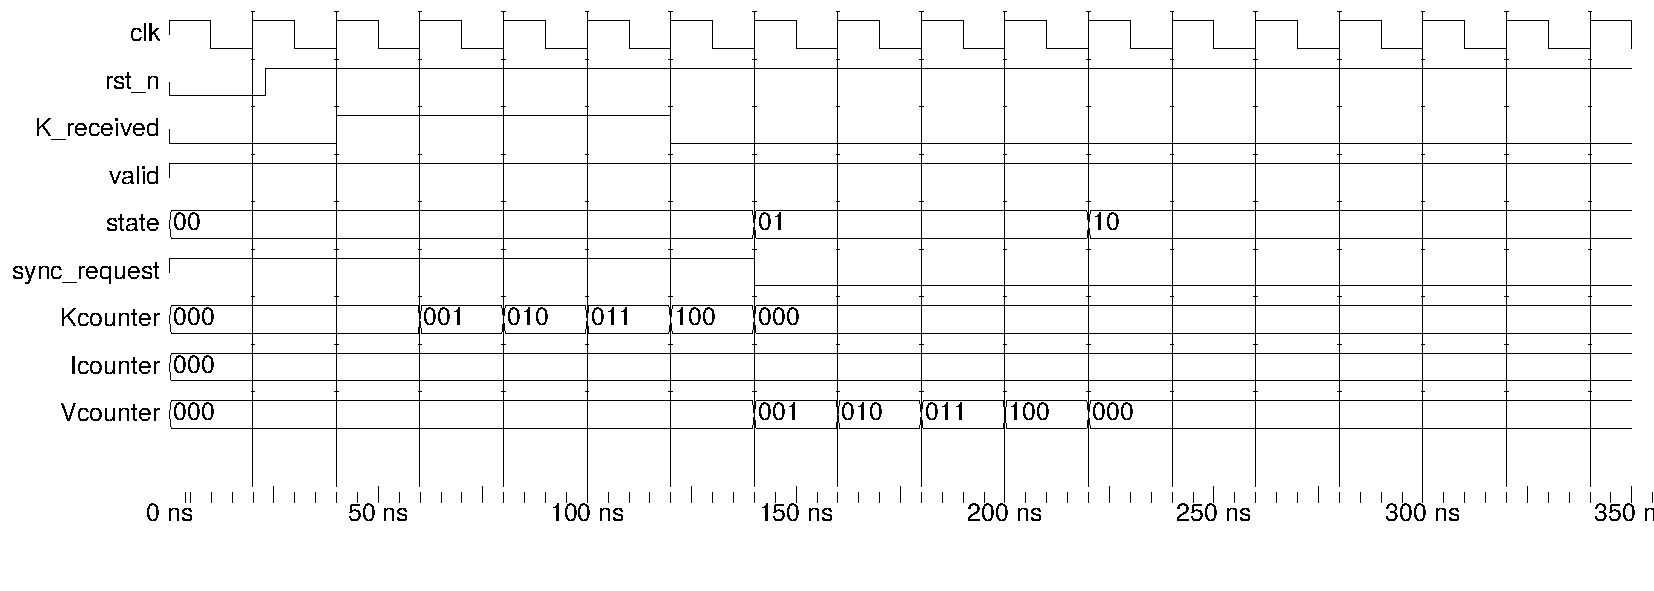
\includegraphics[width=18cm]{./img/cgs_detection_wave.pdf}
	\caption{码群同步仿真结果}
	\label{fig:cgs_detection_wave}
\end{figure}

以上结果是一次正常接收/K/字符的码群同步检测,可以很清楚地看到状态机状态的跳转。
输入信号K\_received表示正确收到一个/K/字符,输入信号valid表示对应字符是有效的字符。
输出信号state即为状态机的输出,可以发现在默认情况下,state以00表示,即为CS\_INIT状态。
在连续收到4个/K/字符后,Kcounter记到100,并在下一个周期状态机跳转到了01状态,即为CS\_CHECK状态。
之后又收到了4个valid的字符后,虽然不一定是/K/字符,但是Vcounter记到100,状态机在下一个周期跳转到了10状态,即为CS\_DATA状态。
实际上,在CS\_CHECK状态和CS\_DATA状态,码群同步已经完成,设置CS\_CHECK状态的主要目的就是在收到过多的invalid字符后需要回到CS\_INIT状态重新进行码群同步。
通知发送端的SYNC~信号改变就需要码群同步状态机提供的sync\_request信号。

\subsubsection{综合}

表\ref{tab:cgs_detection_syn}所示的是码群同步模块的综合结果,分析可以发现,单个lane的码群同步有限状态机可以工作在1GHz左右的频率下,比特速率大约为8GHz。

\begin{table}[H]
\centering
\caption{码群同步模块综合具体结果}
\label{tab:cgs_detection_syn}
\begin{tabular}{|c|r|r|r|}

\hline

\diagbox{项目}{设计} &  码群同步 \\

\hline

Total cell Area($\mu m^2$) & 1586 \\

\hline

Total Area($\mu m$)				&	10033	\\

\hline

Timing($ns$)					   &	8.97 \\

Time Used($ns$)					 & 0.91 \\

\hline

Frequency($MHz$)				&	1098 	\\

\hline

Cell Internal Power($nW$)		&	103.6	\\

Net Switing Power($nW$)			&	15.5 	\\

\hline

Total Dynamic Power($nW$)		&	119.0 	\\

\hline

\end{tabular}
\end{table}

\subsection{初始化帧同步及初始化lane同步}

\subsubsection{仿真}

设计完整功能的初始化帧同步模块仿真结果如图\ref{fig:8b_10b_decoder_wave}所示。

\begin{figure}[H]
	\centering
	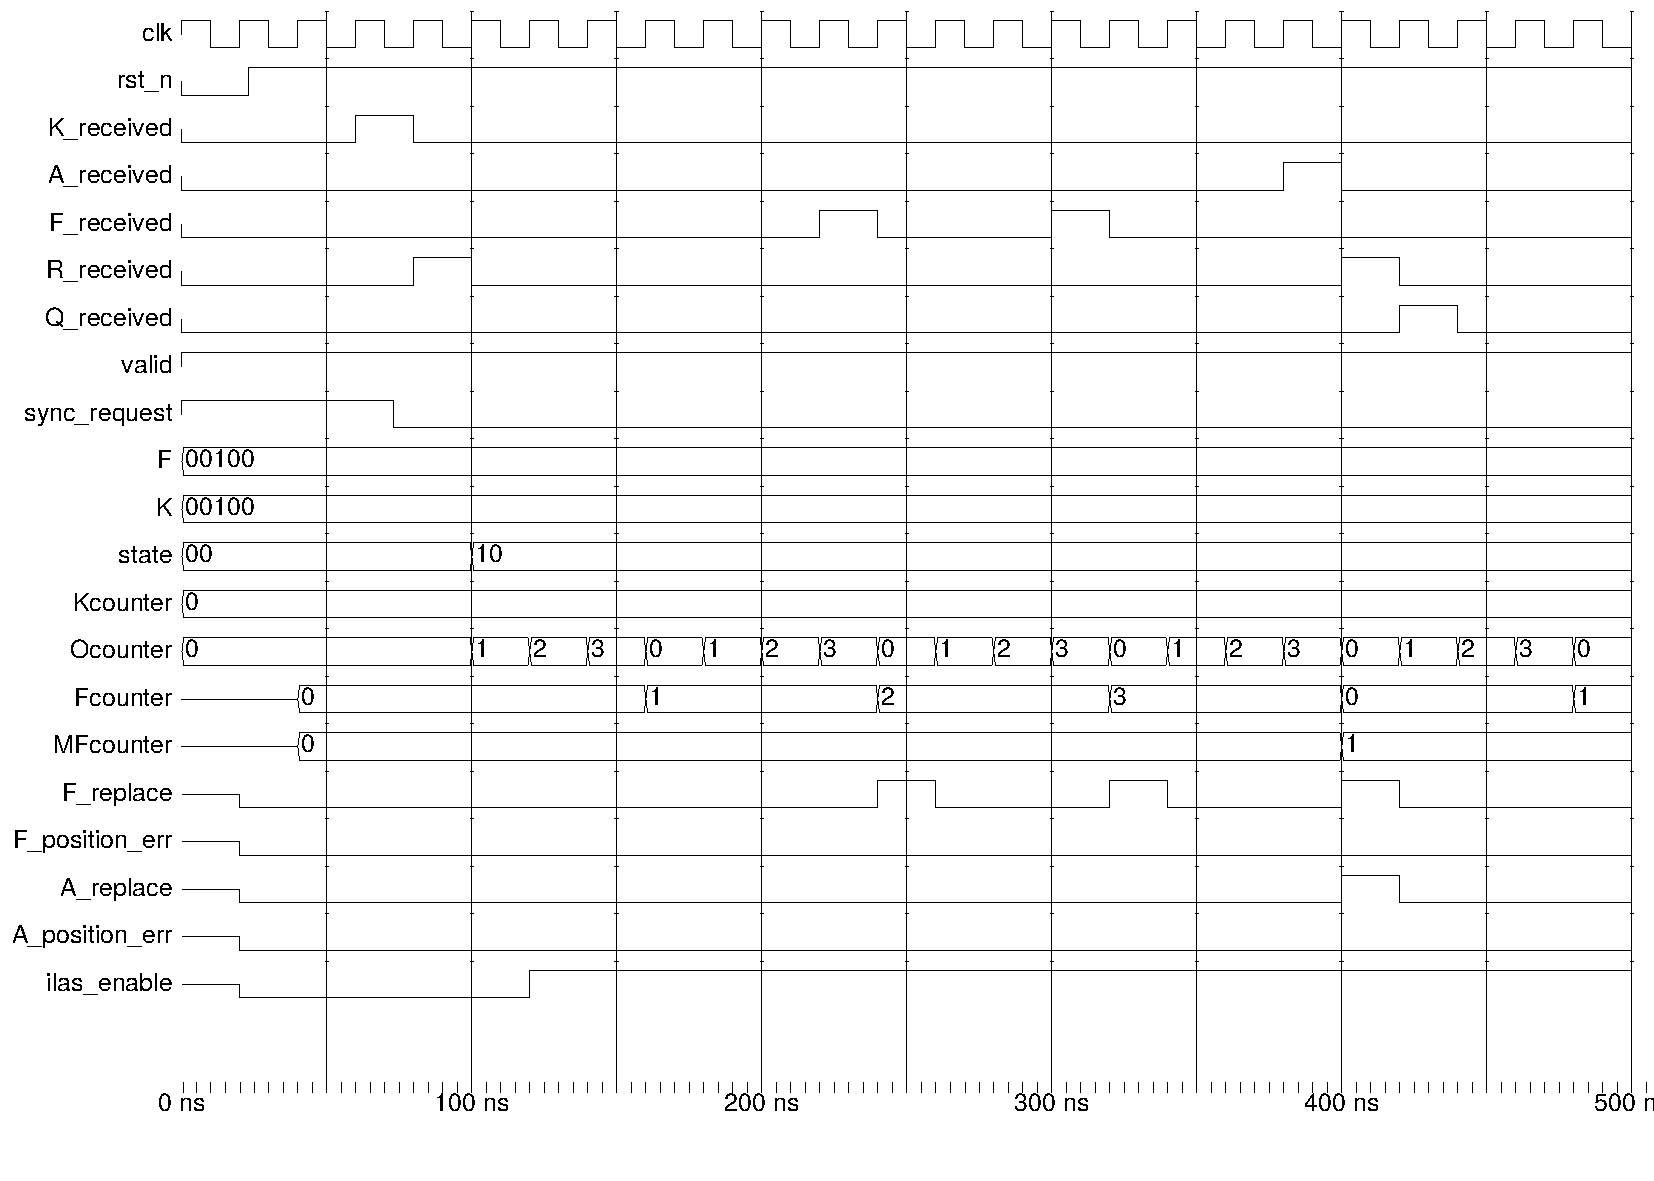
\includegraphics[width=18cm]{./img/ifs_detection_wave.pdf}
	\caption{始化帧同步模块仿真结果}
	\label{fig:ifs_detection_wave}
\end{figure}

以上结果是一次正确的初始化帧同步阶段的仿真结果。
由于篇幅原因,将ILAS检测也融合到了本次结果中。
接收到的信号为控制字符的指示信号,如果不是这五个信号中的一个则为数据信号。
本次仿真的K参数,即多帧中的帧数为4,F参数,即帧中的octet数为4。
可以发现,当复位信号结束后,Ocounter开始以4计数,由Fcounter和MFcounter可以标识出具体的octet在数据流中的位置。
当在帧尾位置收到/F/字符,则会触发F\_replace信号,表示需要替换该字符为上一个帧的数据字符。
当在多帧尾位置收到/A/字符,则会触发A\_replace信号,表示需要替换该字符为上一个帧的数据字符。
MFcounter在收到4个帧后发生累加,说明4个帧组成一个多帧。
由于ILAS需要持续4个多帧周期,所以在本图中无法体现。

设计完整功能的数据流处理模块仿真结果如图\ref{fig:data_flow_wave}所示。

\begin{figure}[H]
	\centering
	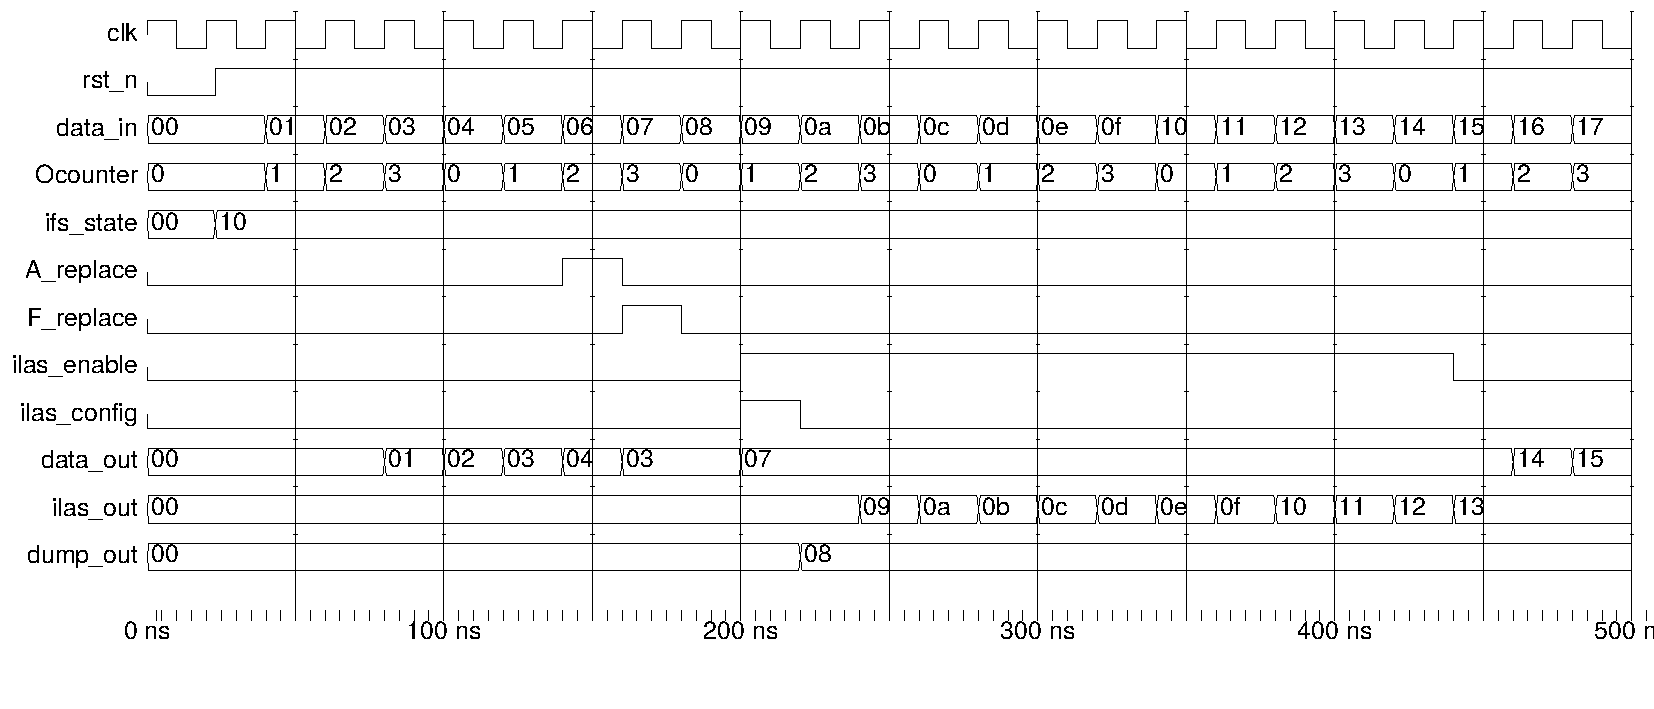
\includegraphics[width=18cm]{./img/data_flow_wave.pdf}
	\caption{数据流处理模块仿真结果}
	\label{fig:data_flow_wave}
\end{figure}

本设计采用的是控制流与数据流分离的设计思路,控制流由之前图\ref{fig:ifs_detection_wave}所示的状态机模块实现。
而本数据流接收模块根据状态机给出的控制信息对数据字符进行替换并选择输出路径。
ILAS数据通过ilas\_out传输到ILAS处理模块,对配置信息进行提取,其控制信号为ilas\_enable信号,当该信号为高电平时,说明该数据流上目前为ILAS配置信息。
当收到A\_replace和F\_replace信号时,输出的信号会进行替换,将上一帧最后一个字符替换到控制字符,以保证输出数据的正确。

最后将初始化帧同步、初始化lane同步和数据流模块级联仿真结果如图\ref{fig:recv_top_wave}所示。

\begin{figure}[H]
	\centering
	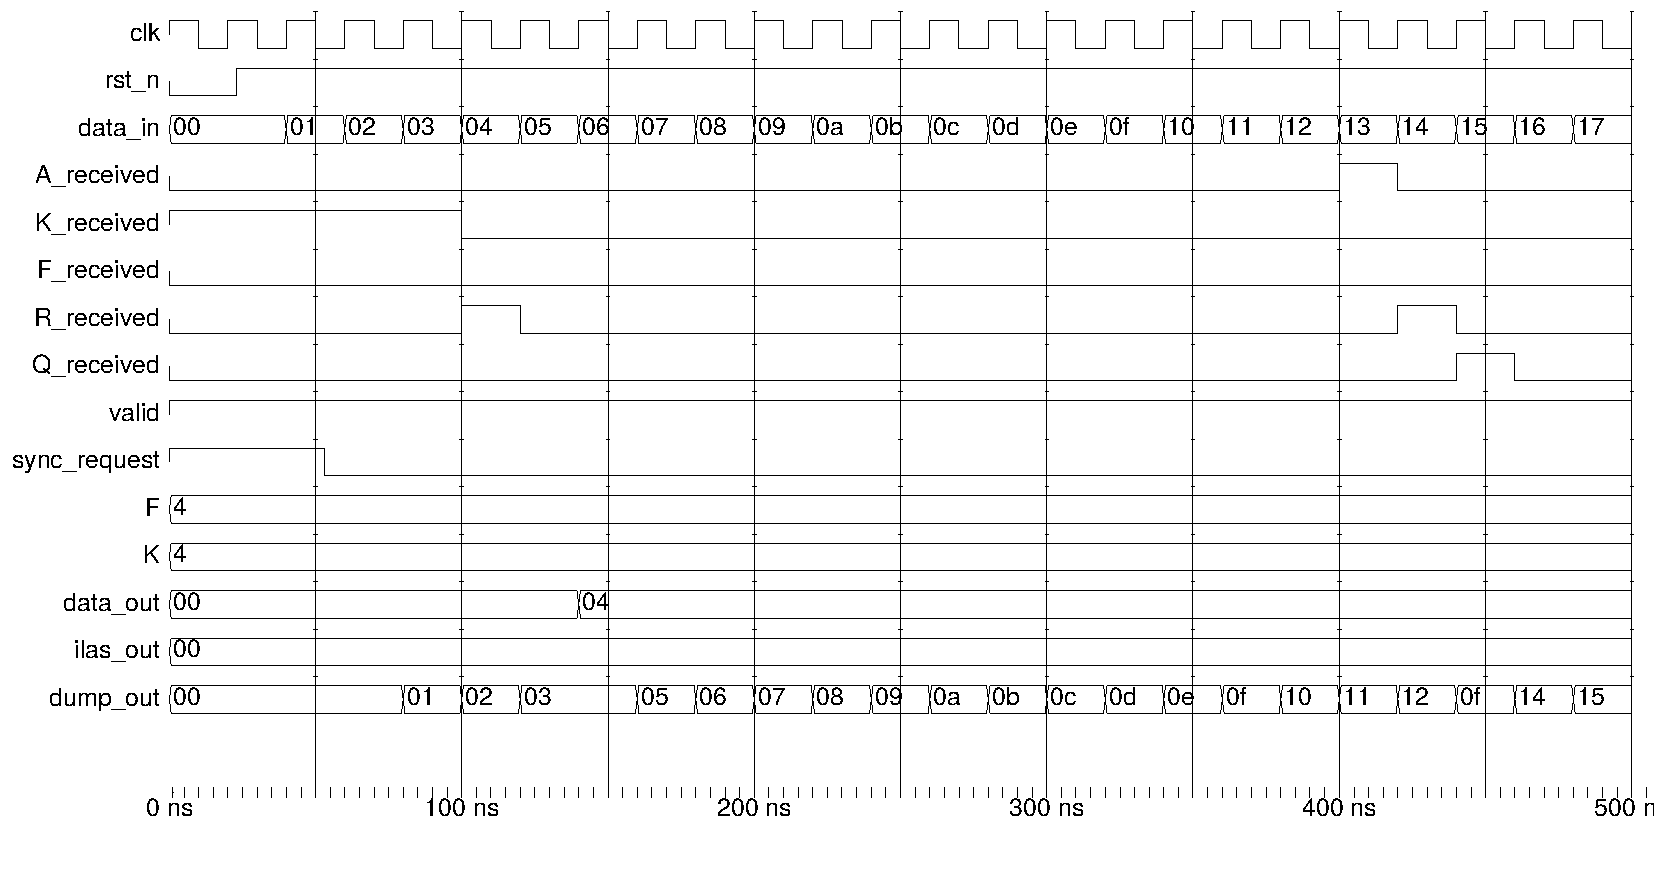
\includegraphics[width=18cm]{./img/recv_top_wave.pdf}
	\caption{级联仿真结果}
	\label{fig:recv_top_wave}
\end{figure}

由于版面限制,只能展示其中一部分信号,模块模拟了完成码群同步后,根据具体信号控制信息的输入,对信号的分配情况。
初始化帧同步首先就是收到了/R/字符表示进入了ILAS序列传输阶段,并检测到一个多帧的最后存在一个/A/字符,根据替换规则,会将该字符替换为上一帧最后一个字符0x0f。
但由于这仍处在ILAS阶段,所以配置信息的字符都会视作无效字符,由dump\_out直接输出,不进入之后的模块。

\subsubsection{综合}

表\ref{tab:ifs_ils_detection_syn}所示的是始化帧同步及初始化lane同步模块的综合结果,分析可以发现,单个lane的码群同步有限状态机可以工作在163MHz左右的频率下,比特速率大约为1.3GHz。
对数据流处理模块分析发现,单个lane可达到的工作频率为502MHz,比特速率大约为4GHz。

\begin{table}[H]
\centering
\caption{模块综合具体结果}
\label{tab:ifs_ils_detection_syn}
\begin{tabular}{|c|r|r|r|}

\hline

\diagbox{项目}{设计} & 初始化帧同步及初始化lane同步模块 & 数据流控制模块 \\

\hline

fa check Area($\mu m^2$) & 1077 &  \\

ifs fsm Area($\mu m^2$) & 6077 &  \\

ilas check Area($\mu m^2$) & 76	&  \\

la check Area($\mu m^2$) & 1067	&  \\

\hline

Total cell Area($\mu m^2$) & 8718 & 4966 \\

\hline

Total Area($\mu m$)				&	51885	& 23819 \\

\hline

Timing($ns$)					   & 3.71 & 7.96 \\

Time Used($ns$)					 & 6.15 & 1.99 \\

\hline

Frequency($MHz$)				&	162.6 & 502.5 \\

\hline

Cell Internal Power($nW$)		&	428.8	& 435.4 \\

Net Switing Power($nW$)			&	96.8 & 55.5 \\

\hline

Total Dynamic Power($nW$)		&	535.6	& 490.9 \\

\hline

\end{tabular}
\end{table}

\bibliography{../../bib/serdes}
\end{document}
